\chapter{Reading notes}

\section{Quotes}

\subsection{Ways of Seeing}

\begin{quotation}
    Having seen this reproduction, one can go to the National Gallery to look at
the original and there discover what the reproduction lacks. Alternatively, one
can forget about the quality of the reproduction and simply be reminded, when
one sees the original, that it is a famous painting of which one has already
seen a reproduction. But in either case, the uniqueness of the original now lies
in it being the original of reproduction. It is no longer what its image shows
that strikes one as unique; its first meaning is no longer to be found in what
it says, but in what it is.
\end{quotation}

\begin{quotation}
This new status of the original work is the perfectly rational consequence of
the new means of reproduction. But it is at this point that a process of
mystification again enters. The meaning of the original work no longer lies in
what it uniquely says but in what it uniquely is. How is its unique existence
evaluated and defined in our present culture? It is defined as an object whose
value depends upon its farity. This value is affirmed and gauged by the price it
fetches on the market
\end{quotation}

\section{Heritage and Conservation}

\subsection{Curated Decay \cite{desilvey_curated_2017}}

If a solution to conservation of historical harpsichords is a part
reconstruction and part re-enactment of the function of the original interface
by creating a new augmented one, then there is still a question of how the new
artefact is conserved as it ages. If the same process is applied where the copy
is preserved and reconstructed, then it is `harpsichords all the way down'.

Reference to \cite{desilvey_curated_2017} will be used as a justification /
motivation for the interface as a finite object, something that is to be `used
up.' The permanent part, the focus for conservation, is not the interface but
the instructions for re-creating it.

DeSilvey speaks mainly towards architecture, the book covers

\begin{enumerate}
    \item Introduction p.1-21
    \item A homestead in Montana
    \item Mullion Harbor, Cornwall
    \item Atomic Weapons Research Establishment (AWRE) facility, Orford Ness
    \item Duisburg Nord Landschaftpark, Ruhr, Germany and Kilmahew, St. Peter’s
    Seminary, Glasgow
    \item An engine house complex, Cornwall; a [former] gunpowder works; an
    abandoned Montana gold mining camp
    \item Lighthouse at Orford Ness decommissioning
    \item Conclusions on Care
\end{enumerate}

\begin{quotation}
    In his discussion of the destruction of a twelfth-century Norwegian church,
    Cornelius Holtorf asserts that processes of change and creative
    transformation may actually help maintain a connection to the past rather
    than sever it.12
\end{quotation}

12 Cornelius Holtorf, “Averting Loss Aversion in Cultural Heri- tage,”
International Journal of Heritage Studies 21, no. 4 (2015): 405– 21.

\begin{quotation}
    The practitioners whom I consulted in the course of this study are acutely
    aware of how the inevitable, inexorable forces of ma- terial transformation
    alter the objects and the places they are responsible for, but in their
    professional roles, they are often obliged to apologize for these changes or
    to pretend that they are not happening, rather than seeing change as an
    oppor- tunity for engaging people and acknowledging vulnerability.
\end{quotation}[][p. 9]

\begin{quotation}
    Archaeologist Siân Jones has argued that the persistent emphasis on
    “material fossilisation” in British and European contexts blinds us to the
    ways in which we also produce meanings through engagement with the dynamic
    social and organic lives of monuments and artifacts. She sug- gests that we
    need to be more open to the processes through which things “grow, change,
    rejuvenate, collapse and decay,” and attentive to the meanings and values
    that are produced along the way.27
\end{quotation}[][p. 9]

27. Siân Jones, “The Growth of Things and the Fossilisation of Heritage,” in A
Future for Archaeology: The Past in the Present, ed. Robert Layton, Stephen
Shennan, and Peter Stone (London: UCL Press, 2006), 113.

\begin{quotation}
The multiplicity that results when maintenance and repair is withheld is the
measure of entropy in the structure, and it is inherently unpredictable and
uncertain.
\end{quotation}[][p. 11]

\begin{quotation}
    Massive amounts of energy are invested to keep heritage systems in a steady
    state so that the matter contained within them will continue to function as
    a cultural mnemonic device. Such work can involve freezing, irradia- tion,
    treating for mold, inserting borate rods, and any number of other preventive
    and protective techniques. In an entropic system, however, matter
    continually degrades, energy is lost, and an element of chance enters into
    the equation.
\end{quotation}

\begin{quotation}
“Entropy is an additive measure of the number of possibilities available to a
system. . . . As the constraints that inform a living organism dissolve, the
entropy of the organism increases. . . . Yet even in the death, new possibili-
ties are sown.”30 
\end{quotation}[][p.11]

30 Don S. Lemons, A Student’s Guide to Entropy (Cambridge: Cam- bridge
University Press, 2013), 160.

\begin{quotation}
    There is a whole field devoted to the study of the biodeterioration of
    cultural heritage, but the focus of scholarship, for the most part, remains
    resolutely fixed on the destructive aspects of the decay process and on
    identifying strategies for protection and remediation.
\end{quotation}[][p. 11-12]

\begin{quotation}
    our handling of the material record that has persisted from the past into
    the present is always a negotiation of the “virtual extremes of total
    preservation and total erasure.”38 
\end{quotation}[][p. 12]

38 Gavin Lucas, “Time and the Archaeological Archive,” Rethinking History 14,
no. 3 (2010): 35

\begin{quotation}
    A focus on entropy allows us to look to the processes by which worlds are
    assembled and to accept that any given system, be it a granite chimney stack
    or an artwork, has the potential to un- fold along multiple trajectories;
    what may appear as erasure on one register may be generative of new
    information on another. An attentive relation to material systems and their
    histories involves following trajectories of change and trans- formation
    rather than arresting them.
\end{quotation} [][p. 12-13]

\begin{quotation}
    we save things not “because they are valued, but rather they are valued
    because they are being saved.”44
\end{quotation}

44 Cornelius Holtorf and Oscar Ortman, “Endangerment and the Conservation Ethos
in Natural and Cultural Heritage: The Case of Zoos and Archaeological Sites,”
International Journal of Heri- tage Studies 14, no. 1 (2008), 

\begin{quotation}
    With each act of preservation, the vulnerable object becomes (a little bit
    of) us, and its unmak- ing threatens to unmake our identities as well.
\end{quotation}

\begin{quotation}
    If memory is understood not as something that is deposited within material
    containers for safekeeping but as something that is “ignited in dialogue
    between mind and matter,” then it does not necessarily need to rely on a
    stable material form for its expression.47
\end{quotation}[][p. 14]

47 Þóra Pétursdóttir and Bjørnar Olsen, “Introduction: An Archae- ology of
Ruins,” in Olsen and Pétursdóttir, Ruin Memories, 9.

\begin{quotation}
    It may be that in some circumstances a state of gradual decay provides more
    opportunities for memory making, and more potential points of engagement and
    interpretation, than the alternative.49
\end{quotation}


49 ``It is also worth mentioning that forgetting, in relation to ideas of the
self, is largely a fiction, and the absent present may re- emerge as a haunting,
the return of the repressed.'' Steve Pile, Real Cities: Modernity, Space, and
the Phantasmagorias of City Life (London: Sage, 2005).

\begin{quotation}
    the anxiety associated with surrender, with allowing processes of change to
    progress unchecked.
\end{quotation}[][p. 15]

\begin{quotation}
    It goes against the grain of human nature to step back and allow things to
    collapse; the urge to step in at the last min- ute to avert material
    disintegration is a powerful one.51
\end{quotation}

51 Elizabeth Spelman, Repair: The Impulse to Restore in a Fragile World (Boston:
Beacon Press, 2003) Main Library 2nd Floor BF636 Spe.

\begin{quotation}
    We need ways of valuing the material past that do not necessarily involve
    accumulation and preservation—ways that in- stead countenance the release of
    some of the things we care about into other systems of significance.
\end{quotation}[][p.17]

\begin{quotation}
    Almost all of the terms that are used to describe attitudes of care, toward
    both cultural artifacts and natural environments, assume the desirability of
    a return to a prior state: restoration, conservation, preservation,
    reconstruction. 
\end{quotation}[][p. 20]

\begin{quotation}
    Cornelius Holtorf and Oscar Ortman: “We prefer . . . a past that is fragile,
cannot be replaced, and needs our help. . . . One might even say that
archaeological sites are not being saved because they are valued, but rather
they are valued be- cause they are being saved.”2
\end{quotation}[Chapter 8][]

2. Cornelius Holtorf and Oscar Ortman, “Endangerment and the Conservation Ethos
in Natural and Cultural Heritage: The Case of Zoos and Archaeological Sites,”
International Journal of Heri- tage Studies 14, no. 1 (2008): 86

\begin{quotation}
    what could be gained if we were to care for the past without pickling it.
\end{quotation}

\subsection{\cite{holzer_imperfect_2025}}

\begin{quotation}
Changes to the object are assumed to diminish that authenticity in some way
\cite{laurenson_authenticity_2006}.    
\end{quotation}

\begin{quotation}
As an example, the policy of the Swedish Museum of Perform- ing Arts is that a
music instrument becomes a historical document upon entering its collection
[23]. Measurement-making is per- mitted in order to ‘read’ these documents, but
playing them is prohibited. Every instrument is preserved in its acquired state,
with no further replacement of parts or repairs of previous dam- ages.
\end{quotation}
They cease to be instruments and become vases.


\subsection{blink of an ear}

\begin{quotation}

This is an argument that has been made before, in many ways and by many people.
Charles Sanders Peirce believed that it is always a matter of relations, of
thirdness. Maurice Merleau-Ponty enlarged Edmund Husserl’s phenomenology beyond
the thing-itself, or even the thing-as-it-appears-in-perception, to include
issues of language, knowledge, and society. Rosalind Krauss seized upon
Merleau-Ponty’s expansion, identifying the art-historical turn away from an
emphasis

on material and perception to a concern with the discursive frameworks that
authorize, motivate, and define a field of practice. What Krauss identifies as
the transition to postmodernism, Peter Osborne sees as the conceptual turn to an
art that questions its own ontological and epistemological conditions. Such
reconceptions of art’s status appeal to the innovations of poststructuralist
thought, notably that of Jacques Derrida and the revolutionary reformulation of
meaning as the product of the trace of alterity in the apparent self-sameness of
the thing-itself. Derrida diagnoses the uncontainable differential processes at
work in the constitution of the it and thus establishes the absence at the heart
of what appears to be presence. The thing-inquestion cannot be satisfactorily
pinpointed or contained. It cascades outward formlessly and infinitely,
necessitating an aesthetics of the sublime rather than of beauty. According to
Jean-François Lyotard, such an aesthetic is characteristic of the postmodern
condition. Kim-Cohen, Seth. In the Blink of an Ear : Toward a Non-Cochlear Sonic
Art, Bloomsbury Academic \& Professional, 2009. ProQuest Ebook Central,
http://ebookcentral.proquest.com/lib/ed/detail.action?docID=601811. Created from
ed on 2025-07-21 11:08:20.

\end{quotation}

`Thirdness' in Blink of an Ear, Context of the van gogh painting in Ways of
Seeing \cite{berger_ways_1972} and

\subsection{\cite{mcluhan_understanding_1964}}

\begin{quotation}
In a culture like ours, long accustomed to splitting and dividing all things as
a means of control, it is sometimes a bit of a shock to be reminded that, in
operational and practical fact, the medium is the message. This is merely to say
that the personal and social consequences of any medium — that is, of any
extension of ourselves — result from the new scale that is introduced into our
affairs by each extension of ourselves, or by any new technology.
\end{quotation}
\cite{mcluhan_understanding_1964}

\subsection{\cite{laurenson_authenticity_2006}}

\begin{quotation}
minimising change to the physical work means minimising loss, where loss is
understood as compromising the (physical) integrity of a unique object
\end{quotation}

\begin{quotation}
Any discussion of damage or loss quickly moves into the realm of ontology in the
need to define change against something perceived as the identity of the work.
The conservation object is still largely an object of the Enlightenment, an
object that can be known through scientific analysis. A traditional
‘conservation object’ is an object which has been studied scientifically and for
which has been established what is known as its ‘state’. ‘The term ‘state’ is
intended as a description of everything that can be defined or discovered about
an object by observation, measurement or analysis. It is an attempt to define
properties that are intrinsic, objective, impersonal, and in distinct contrast
to the properties of ‘value’.19

Within this conceptual framework, change is understood with reference to the
state of the object, and change that is irreversible and undesirable is defined
as damage or loss. For traditional conservation the identity of the work is
understood in terms of its material identity and this is considered the proper
focus of conservation. It operates within a scientific paradigm where the
conservator carefully avoids being lulled into interpretation. The practice
associated with interpretation is restoration, which is seen as essentially
unscientific and rather frivolous or unprofessional. In this model the
conservation object is a unique object, which contains material evidence that
enables authentication. Such objects are collected by museums as the ‘tangible
traces left by our ancestors.’ 20
\end{quotation}


\begin{quotation}
What is emerging is a conceptual dependency between the ontological framework in
which an object is classified and described and the attending concept of
authenticity. If the ontological framework is focused on the material so will
the notion of authenticity. If the ontological framework shifts, then we expect
a similar shift in our concepts of authenticity, change and loss.
\end{quotation}

The musical instrument also has authenticity in terms of `sound'. Two
instruments can be constructed by the same maker and have vastly different
sounds due to differences in material properties. Similarly, a copy of an
instrument might only be considered authentic if the sounds were the same.

(side note, newer instruments look differen unless they aged or have a
artificial patina applied to them. as shown by \cite{fritz_player_2012} and
\cite{tsay_sight_2013} the visual has a great impact on aural perception)

\begin{quotation}
The conceptual framework of traditional fine art conservation is focused on
material objects that can be known through scientific analysis and that contain
evidence of authenticity and of the hand of the artist. The material object is
the root of an aesthetic experience and the conservator is charged with being
true to the ‘original’ work. As I have previously suggested, this conceptual
framework does not sit well with time-based media installations which are in
part, both temporal and ephemeral. In what follows I shall look to the
philosophy of music to explore alternative ways of understanding authenticity,
change and loss in ways that might help to guide the conservation of these works
of art.
\end{quotation}

Shown by Fritz in \cite{fritz_listener_2017}, instruments quality should be
considered ephemeral as degradation in quality is terminal after 2 years.


\begin{quotation}
They are similar to works that are performed, in that they belong to the class
of works of art, which are created in a two-stage process. They share this
feature with western notated music where what is experienced is the performance.
Similarly, in the case of a time-based media installation, the work must be
experienced as an installed event, which again has parallels with a performance.
\end{quotation}

\begin{quotation}
The kinds of things that might act as work-defining properties of a time-based
media installation are: plans and specifications demarcating the parameters of
possible change, display equipment, acoustic and aural properties, light levels,
the way the public encounters the work and the means by which the time-base
media element is played back.
\end{quotation}

The medium is the message, media is not just the work but how it was diffused.
So much of early video work engaged with the aesthetics of CRT monitors that it
would be considered in authentic (by whom) to use any other technology. CRT
monitors are no longer widely produced.

\begin{quotation}
In the tradition of Western music, works have a score and for the philosopher
Stephen Davies, this is ontologically significant: ‘a performance of a given
work is authentic if it faithfully instances the work, which is done by
following the composer’s work-determinative instructions as these are publicly
recorded in its score.’25

A score, according to Davies, is a notation that has the function of specifying
works. A score is intended as instructions to potential performers and ‘it is by
following these instructions that players generate instances of the work.’26
Davies also believes in an account of the ontology of musical works which links
them to their historical context: ‘the proper interpretation of a score requires
knowledge both of conventions for the notation and of the performance practice
shared by the composer with the musicians to whom the score is directed.’27
Performances can occur in different times and different places with different
performers and still be authentic instances of that performance. In the
performance of a musical work it is recognised that there is a gap between a
work as represented as a score and its performance. This allows us to speak of
good and bad performances while still being able to say that a work is the same
work even if badly performed. There is room for interpretation.
\end{quotation}

Rebuttle: There is still value judgement to be made with respect to music. Are
the instruments period appropriate, not just in form but also material. There is
also tuning and acoustics and setting all of which can be impractical to
reproduce. It is not just historical instruments. Is a performance authentic if
unless it uses an original 1964 Moog synthesizer. Countless nuances in the
fabrication process and materials have at least a self-perceived impact on the
quality of the sound. Is `authenticity' of sound a constructive metric with
which musical instruments can be measured.

(what may not be important to one person is important to another and considering
the process of conservation choices need to be deliberate).

TODO: Read Davies full article

\begin{quotation}
Authenticity in this context means an obligation for the museum or custodian to
faithfully realise those aspects of the work which are important to its meaning.
In the fullest sense this includes historical accuracy, although in a fine art
context aesthetic concerns will take priority over the historical. It is
possible for two performances or installations of a work to differ but both be
authentic. Only if a composer’s or artist’s instructions determined every aspect
of an installation would there be only one possible way in which an authentic
performance or installation could be rendered. But in such cases the element of
performance would be diminished. They would be more akin to painting and
sculpture because their realisation would not be a two-part creative process but
would rather be like decoding a recording – a mechanical process.
\end{quotation}

In the same as aesthetic concerns might trump historical accuracy, with musical
instrument we might consider addressing the authenticity of \textit{experience}
over form.


\begin{quotation}
\begin{quotation}
The Steinway grand, with its metal frame and sturdy construction, easily
survives its use in a performance of Beethoven’s Appassionata. When one hears
that work on a period fortepiano, the impression is very different. Then it
becomes easy to appreciate the stories about the rate at which Beethoven broke
pianos, for it is apparent that the instrument is deliberately pushed to its
limits in the sonata. It sounds as if it might be shaken to bits by the fury of
the music.33
\end{quotation}
In claiming video, film, slide etc. as an artistic medium, artists too may push
the limits of the technology and display devices and create an experience very
different at the time in which the work was made to how it might be experienced
today.

The issue of display equipment has been addressed in more detail elsewhere.34
In brief, I believe that it is possible to place both an inappropriately high
and low level of significance on the association of a piece of display equipment
with a time-based media work of art. The issue of authority in decisions of this
sort is complex, and we have already discussed the possibility of two authentic
installations that are different. Nevertheless, it is clear that certain
considerations operate as candidates for criteria for such decisions and others
do not.
\end{quotation}

Imagine a performance art piece whose instructions were for a performer to stand
in a gallery and smash a Stradivarius violin.


The focus is on musical performance, which may or may not include historical (or
reproductions of historical) instruments. Experience of use is still left
unexplored.

\subsection{\cite{salvador_contemporary_2005}}


As Muñoz Viñas (2003) has put it, classical theories contemplate conservation as
a ‘truth-enforcement’ operation. Although they do not agree upon exactly where
that truth resides, since its very inception, the main purpose of conservation
is to maintain or reveal an object’s true nature or integrity (see, for
instance, UKIC, 1983; Fernandez-Bolaños, 1988; Caple, 2000; Clavir, 2002). p65


\begin{itemize}
    \item UKIC (United Kingdom Conservation Institute) (1983). Guidance for
    Conservation Practice. London: UKIC
    \item Caple, C. (2000). Conservation Skills. Judgement, Method and Decision
    Making. London: Routledge    
\end{itemize}



\subsection{\cite{avrami_values_2000}}

David Thorsby in Economic and Cultural Value in the Work of Creative Artists
lists values of

\begin{itemize}    
\item aesthetic value: beauty, harmony;
\item spiritual value: understanding, enlightenment, insight;
\item social value: connection with others, a sense of identity;
\item historical value: connection with the past;
\item symbolic value: a repository or conveyor of meaning.
\end{itemize}

\begin{figure}
    \centering
    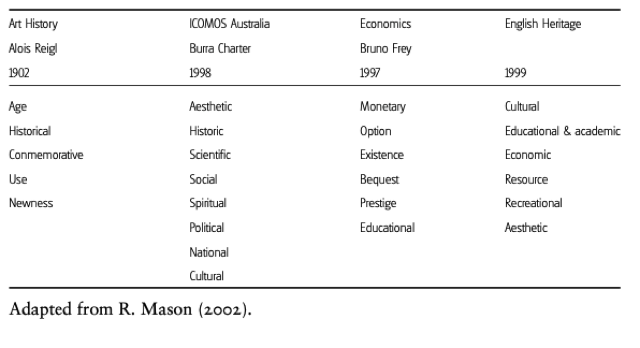
\includegraphics[width=1\linewidth]{img/values.png}
    \caption{from \cite{torre_values_2013}}
    \label{fig:enter-label}
\end{figure}

\begin{table}[h]
    \centering
    \resizebox{\textwidth}{!}{
    \begin{tabular}{llll}
        \toprule
        \textbf{Art History} & \textbf{ICOMOS Australia} & \textbf{Economics} &
        \textbf{English Heritage} \\
        Alois Reigl & Burra Charter & Bruno Frey &  \\ 
        1902 & 1998 & 1997 & 1999 \\ \hline
        Age& Aesthetic& Monetary & Cultural\\ 
         Historical &  Historic&  Option &  Educational and academic \\ 
         Commemorative& Scientific& Existence & Economic\\ 
         Use&  Social (including spiritual, political, national, other
cultural)&  Bequest &  Resource \\ 
         & & Prestige & Recreational \\
         & & Educational & Aesthetic\\
    \end{tabular}}
    \caption{Comparative Analysis of Value Systems}
    \label{tab:values_comparison}
\end{table}

\begin{table}[h]
    \centering
    \begin{adjustbox}{width=\textwidth}
        \begin{tabular}{llll}
            \toprule
            \textbf{Art History} & \textbf{ICOMOS Australia} &
            \textbf{Economics} & \textbf{English Heritage} \\
            Alois Reigl & Burra Charter & Bruno Frey &  \\ 
            1902 & 1998 & 1997 & 1999 \\ \hline
            Age& Aesthetic& Monetary & Cultural\\ 
             Historical &  Historic&  Option &  Educational and academic \\ 
             Commemorative& Scientific& Existence & Economic\\ 
             Use&  Social (including spiritual, political, national, other
    cultural)&  Bequest &  Resource \\ 
             & & Prestige & Recreational \\
             & & Educational & Aesthetic\\
        \end{tabular}
    \end{adjustbox}
    \caption{Comparative Analysis of Value Systems}
    \label{tab:values_comparison}
\end{table}


\begin{table}[h]
    \centering
    \begin{adjustbox}{width=\textwidth}
        \begin{tabular}{llll}
            \toprule
            \textbf{Art History} & \textbf{ICOMOS Australia} &
            \textbf{Economics} & \textbf{English Heritage} \\
            Alois Reigl & Burra Charter & Bruno Frey &  \\ 
            1902 & 1998 & 1997 & 1999 \\ \hline
            Age& Aesthetic& Monetary & Cultural\\ 
             Historical &  Historic&  Option &  Educational and academic \\ 
             Commemorative& Scientific& Existence & Economic\\ 
             Use&  Social &  Bequest &  Resource \\ 
             & & Prestige & Recreational \\
             & & Educational & Aesthetic\\
        \end{tabular}
    \end{adjustbox}
    \caption{Comparative Analysis of Value Systems}
    \label{tab:values_comparison}
\end{table}

What is missing from the above, or under emphasised by educational , is
\textit{instructional} use. That is to say, conservation of objects to instruct
in practice which is a function withheld from musical instrument when use is
restricted.

\subsection{\cite[p. 206–253]{davies_authenticity_2001} }

Authentic is a tricky word and should be avoided, espcially in conservation
policy. In summary, it is difficult to tell when Davies is holding a position
held by someone else in order to discuss it or if Davies is putting forth his
own position. The only clear position is \textit{authenticity is impossible to
achieve in principle}.

Harpsichord Interface does not argue for an \textit{authentic} experience, there
are many parts of it which are in authentic, but rather towards a true or
comparable experience from which a player can learn and react to the tactile
response.

Authenticity or fidelity of a work should not be conflated with authenticity of
an object.

\begin{quotation}
As a first response, one can query the equation of change with improvement
(Godlovitch 1988). Period instruments often had many distinctive and endearing
qualities that were sacrificed in the name of progress and uniformity. The
wooden Baroque flute has a warm intimacy of tone that is absent from its modern,
metal counterpart. Harpsichords possessed stops and allowed for octave
couplings, whereas pianofortes lack these. The fortepiano had a lighter, drier
tone than the felt‐hammered, modern grand. Some fortepianos had harp, bassoon,
and Turkish stops (Kirkby 1966: 23). With its flatter bridge, the Baroque violin
was more suited than the modern instrument to double stopping. Moreover, the
wide variety among instances of cellos and oboes, for instance, allowed for a
more subtle matching of instrument to work than is now possible.

The following also points to the danger of assuming that the ‘improved’ version
is the better one to use: the Steinway grand, with its metal frame and sturdy
construction, easily survives its use in a performance of Beethoven's
‘Appassionata’. When one hears that work on a period fortepiano, the impression
is very different. Then it becomes easy to appreciate the stories about the rate
at which Beethoven broke pianos, for it is apparent that the instrument is
deliberately pushed to its limits in the sonata. It sounds as if it might be
shaken to bits by the fury of the music. One might compare this experience with
watching two cars travelling down a road at the same speed. One is a Rolls
Royce, cruising comfortably in something less than its highest gear, whereas the
other is a Model T Ford, running at the limits of its engine's capacity and on
the verge of blowing a gasket. Though both vehicles progress at the same rate,
their motion appears very different to the person who is aware of their
respective capabilities. That of the Model T is strained and dramatic, whereas
the Rolls's is not. Returning now to the musical case, even if the sounds
produced by the fortepiano and the Steinway were the same (which they are not,
of course), they should sound different to the informed listener, and that
difference would bring out an important feature of the music in the one instance
that was lost to the other. (Kerman 1989 makes a similar observation in
discussing performances of Mozart's piano concertos.)
\end{quotation}

Davies mythologising the older instrument not constructive. Also, presented here
is a false dichotomy between a new instrument and an old instrument.

The fortepiano is also not a fixed design and could very much just be described
as "the piano in development". References to usage of stops or otherwise would
need to be explicit or known to be used by a composer before they could be
considered



\begin{quotation}
    As indicated already in the discussion of the ‘Appassionata’, it might even
    be a virtue in the period instrument that the music seems to threaten its
    structural integrity.
\end{quotation}

Emphasis on the threat to `structural integrity' which over reliance on musical
apocrypha       


\begin{quotation}
As I have already made clear, I agree with Levinson on many of the relevant
issues. We both think the use of appropriate period instruments is essential in
achieving the highest degree of authenticity if their use is required by the
composer. And I concur that some of the properties of musical works depend on
the manner in which the sounds are elicited from the instruments in question.
Where composers conceive their works for performance on specific kinds of
instruments and issue determinative instructions that this be done, these are
properties of the work, not solely of its performances. Though we share these
conclusions and assumptions, Levinson and I differ in our arguments. He is
inclined to suggest that there always is a gestural quality specific to playing
the instruments in question, and that this affects the expressive properties of
the resulting sound, though the perception of these properties is available only
to the listener who is suitably informed about characteristics of the
instruments in question. Also, he takes account of composers' expressed
preferences. By contrast, I doubt that there always are relevant differences
between the expressive character of performances using authentic and inauthentic
instrumentations, and I am concerned with only those intentions of the composer
that the musical practice of the day recognizes as work determinative. It was
not always the case that composers' wishes as regards the instrumentation of
their works were mandatory. Some of those earlier disagreements return in
considering a question that is central to this chapter: is the use of period
instruments, as against their modern equivalents, required for the fullest
degree of authenticity in performance?

\end{quotation}

This may be addressed later, but there is again this supposition that
authenticity is there to server the artist's intent and or the audience
experience / enjoyment. There is still something to be said for the impact on
the performer and what they can learn/

Emphasis on the '


\begin{quotation}
Levinson accepts the challenge, but he does not spell out how the manner of
playing differs in the case he considers.
\begin{quotation}
The musical gestures in Mozart's Thirty‐ninth Symphony, K. 543. . .are
presumably precisely those that are readily perceived in it against the matrix
of the gestural repertoires and sonic capacities of just the instruments for
which the piece was conceived—e.g., old‐style clarinets. . .even if modern
clarinets. . .could produce sounds indistinguishable from those that
eighteenth‐century clarinets would make in rendering the score of Mozart's
Thirty‐ninth Symphony, such a performance would not be expressively equivalent
to any performance achievable on those older, and different, instruments. What
expressiveness it would have is hard to say, bastardy being no simpler to deal
with in the aesthetic realm than in the social one. But in any event, it would
not quite be a proper representation of K. 543's own expressiveness, and hence
not an authentic performance of it. (Levinson 1990c: 407)
\end{quotation}
\end{quotation}

Perhaps what Levinson is driving at here is that the sounds may be identical,
but the effort and motion required to arrive there is very different. Reminder,
the medium is the message.

\begin{quotation}
(Levinson allows, though, that the departure from ideal authenticity involved in
using modern clarinets is a matter of degree and is not so serious as would be
the substitution of an electronic synthesizer for the clarinet.)
\end{quotation}
Interesting philosophical question to Levinson. What if the an instrument had
\textit{expressive equivalency}, but made entirely different sounds to the
original?

Note: something to be said about making a deliberate choice, make it logistical
easier to make that choice.

\begin{quotation}
Because I doubt that the playing of period instruments always requires different
actions from those made in working with their contemporary equivalents, I am
unconvinced by Levinson's argument. For instance, the gestures involved in
sounding the modern pedal tympani cannot be very different from those in playing
its non‐pedal predecessors. Nevertheless, as before, I approve of the conclusion
he draws: that the use of period instruments is required for the fullest degree
of authenticity (given that their use is made work identifying by the composer).
\end{quotation}

`I reckon...' is not a convincing argument, and as was shown in
\cite{fontana_musical_2018, charalampos-saitis_musical_2018,
merchel_musical_2018} vibro-tactile feedback, which would change for instrument
with different mechanics for excitation, impacts the musicians perception of the
sound during performance.

\begin{quotation}
If not by Levinson's argument, how is that conclusion supported? In the first
place, one can appeal to the fact that period instruments usually sound
different from their modern counterparts. Here is just one example:

[Beethoven's Symphony No. 1, Op. 21] calls for clarinets and horns in C. Neither
of these instruments is common today, and the modern substitutes sound quite
different, particularly the horns. The other instruments have also undergone
changes to a greater or lesser extent. . .In addition, there is the problem of
the relative weight of sound between the winds and the strings. Not only have
the actual instruments and manner of playing them changed, but the proportion in
the number of players between the families of instruments have changed. Playing
the score in the modern orchestra, then, is only an approximation of the sound
as Beethoven conceived it. (Silliman 1969: 106)
\end{quotation}

\begin{enumerate}
    \item Levinson, and Silliman, are conflating orchestration and with
    instrument form
    \item ``Modern substitutes sound quite different`` needs to quantified    
\end{enumerate}

\begin{quotation}
It is relevant to add a second observation to this first: period instruments,
when played in the style of the day, sound different from modern ones, but, as
well, they sound better. They make clearer or more salient features of the work
that are aesthetically significant. The quotation at the beginning of this
chapter from Ton Koopman illustrates the point.
\end{quotation}

\cite{fritz_listener_2017} suggests very differently.

\begin{quotation}
Playing harpsichord music on the piano was simply not satisfying—which
eventually led me to take up the harpsichord. Something similar seems often to
be the case with violinists. There are certain things which one finds in early
violin methods which the modern violin and bow are simply incapable of doing.
During my first conservatory years I was involved in a small baroque ensemble,
using modern instruments. The necessity of playing on early instruments became
more and more clear to us; it was not the public which demanded this, but rather
our own growing dissatisfaction. For us, the early instruments began where the
modern ones left off. This also became clear to me while working with musicians
in a modern orchestra; even the most outstanding results do not come close to
what one can achieve on baroque instruments.

(Koopman 1987: 4)
\end{quotation}


Instruments are not discrete designs but rather incorporate changes over time. 

Harpsichord to piano is quite a leap, and is a comparison to apples and oranges.

[Confirmation needed] Baroque violin on the other ha d is a incredibly unfixed
descriptor with variations in body design and scale length. The cremonese
violins are also used as the basis for the design of modern violins. Comparing
two violins a few centuries apart but near identical design save chin rests and
fine tuners against two keyboard instruments with wildly different excitation
mechanics is not a fair comparison. 

\begin{quotation}
Where the change in instrumentation, and adaptations made to the music in the
light of this, are significant, the result is a work transcription that is
distinct from its model. One does not transcribe a work merely by crossing out
the word ‘harpsichord’ on the score and replacing it with ‘piano’ (Davies
1988a), however. Neither does the substitution of the modern cello for its
Baroque cousin result in a work transcription. If Domenico Scarlatti's sonatas
are harpsichord specific, or if Bach's solo cello suites take part of their
identity from their instrumentation, playing them on the piano or the modern
cello will be less than ideally authentic. This is not to say that such
renditions are heinous. There can be good reasons for the substitution. And the
resultant lowering of authenticity might be relatively insignificant.
\end{quotation}


Same story, is \textit{Baroque Cello vs modern Cello is the same as Harpsichord
vs Piano} an equal comparison? One of is a comparison of degree the other is a
comparison of kind.


\begin{quotation}
I claimed that a performance can be ideally authentic even if it cannot be
ex‐perienced by today's listener as it would have been by the original audience.
I did allow, though, that we would not value authenticity as we do unless, in
general, it leads to a greater appreciation of the works that are played.
\end{quotation}

Again, only with respect to the audience, never the performer.



\Subsubsection{Clarification}

Davies clarifies in 

\begin{quotation}
    A highly
authentic performance is likely to be one using instruments contemporary to
the period of composition (or replicas of such instruments) in its performance
\end{quotation}

Is a replica sonically authentic to Davies?

\subsection{\cite{laurenson_management_2005}}

Taking the definition of time-based media installations from
\cite{laurenson_management_2005} and what we know of musical instrument
impermanence from \cite{fritz_listener_2017} we could define musical instruments
as a kind of Time-based creative tool. A very roundabout way of simply equating
musical instruments with anyother tool.

If instruments are a tool, if there value does extend beyond those in the table
above to also include instructions then there must be a means to use it as well
appreciate it.

\cite{laurenson_management_2005} considers how to evaluate equipment used in
time-based media installations.

\begin{quotation}
    Most display equipment is mass-produced and unless modified or rare it is
    not valued for uniqueness and can be substituted with the same make and
    model creating little or no discernible change. When exact substitution is
    impossible and change occurs, the change is assessed by considering the
    significance of equipment to the installation.
\end{quotation}

This simply moves the problem to a point in the future, eventually value will
overtake function. Historical musical instrument have reached that point in the
future where all components are high value and present yet another Ship of
Theseus problem.

\subsection{\cite{jorda_instruments_2004}}


\begin{quotation}
An acoustic instrument consists of an excitation source that can oscillate in
different ways under the control of the per- former, and a resonating system
that couples the vibrations of the oscillator to the surrounding air. Parts of
the per- former’s body transmit the energy for the excitation to the instrument,
interacting through the instrument’s control inter- face. However, in most
acoustic instruments (apart from organs and several other keyboard instruments),
this separa- tion between the control interface and the sound-generating
subsystems is fuzzy and unclear (Hunt et al., 2000; Wanderley, 2001).
\end{quotation}

polyphonic instruments have always had limited continuous control possibilities
\begin{itemize}
    \item Pressing, 1990; Cybernetic Issues in Interactive Performance Systems
    \item Rubine \& McAvinney 1990; Programmable Fingertracking Instrument
    Controllers.
    \item Vertegaal \& Eaglestone, 1996; Comparison of input devices in an ISEE
    direct timbre manipulation task
    \item Levitin et al., 2002 Control parameters for musical instruments: a
    foundation for new mappings of gesture to sound.
\end{itemize}

physical and cognitive limitations of humans and not in the inherent properties
of the instruments
\begin{itemize}
    \item Fitts, 1954;  The information capacity of the human motor system in
    controlling the amplitude of movement
    \item Miller, 1956; The magical number seven plus or minus two: some limits
    on our capacity for processing information
    \item Fitts \& Posner, 1967; Human Performance
    \item Cook, 2001) Principles for designing computer music controllers.
\end{itemize}


\subsection{\cite{uoe_collections_2020}}

How many harpsichords do you need before you stop caring if one of them breaks?

Apparently, ones specifically missing from the collection. With respect to the
harpsichord collection:

\begin{quotation}
    this division is of international importance, and allows a rich and varied
    display of harpsichord family instruments.  The collection is generally
    considered to have the widest scope of any in the world. Each item is
    important for reasons relevant to research and teaching, and in some cases
    performance potential. 
\end{quotation}

With performance potential only becoming less likely as time moves on.

\subsection{\cite{barclay_care_1997}}

\begin{quotation}    
The central theme of this book is managing the retirement of historic musical
instruments from active service
\end{quotation}

\subsubsection{Ethics and the Use of Instruments}

\begin{quotation}
    Musical instruments are similar to other functional objects because they
    have moving parts, or require physical interaction to fulfil the purposes
    for which they were made
\end{quotation}

\begin{quotation}
    Musical instruments, clocks, small craft and . ships, automobiles, arms and
    armour, hand tools, furniture, and indus- trial machinery are typical of the
    wide variety of functional objects found in museums and private collections.
    In most history museums, function- al objects predominate.
\end{quotation}

\begin{quotation}
    there is always pressure from collectors and musical instrument makers, the
    general public, and from many museum staff to restore them to play- ing
    condition so that their musical qualities can be appreciated- in the words
    of one museum direct01~ "to take them out of their glass cases and let them
    sing." 
\end{quotation}

\begin{quotation}
    the educational and aesthetic value of such use is often undeniable, but the
potential for wear and tear, and loss of origi- nal substance is equally great.
\end{quotation}

\begin{quotation}
    Restoration work, though always well intentioned, has often been detrimental
    to the long-term preservation of the instruments, and is considered by many
    to be inconsistent with stan- dards of practice long accepted for other
    classes of museum collections, such as paintings and fine arts.
\end{quotation}

\begin{quotation}
    Even in the case of museum instruments for which restoration to playability
    seems an appropriate option, it is always much more easily proposed than
    safely executed.
\end{quotation}

\begin{quotation}
Factors against Functional Restoration There are a number·of factors that arg\ue
against functional restoration:
    \begin{itemize}
        \item The instrument is unique.
        \item The instrument has original ephemeral features that will be lost
        or altered.
        \item The function is obscure and unlikely to be determined as a result
        of restoration.
        \item The condition of the instrument is such that an accurate
        achievement of its original quality of function is unlikely.
        \item The function is so well understood that no new information is
        likely to be gained.
        \item The instrument is fragile or subject to significant wear during
        use.
        \item Theuseofacopywouldbepossible.
        \item The skills and other resources required for restoration,
        subsequent ongoing maintenance, and use consistent with historically
        appropriate standards are unavailable or only marginally available. ·
        \item The resulting functional use will be not be recorded in any
        permanent form accessible to others.
    \end{itemize}

    Factors for Functional Restoration On the other hand, there are some factors
that favour functional restoration:
\begin{itemize}
    \item The instrument is mass-produced, and many similar examples exist.
    \item The instrument has been previously restored and most ephemeral
    features have already been lost.
    \item The instrument can be easily put into working condition without loss
    of substance or ephemeral features such as adjustments and clearances.
    \item The original function can be reestablished, and useful information
    about it is expected to be gained as a result.
    \item The instrument is sturdy, durable, and not subject to significant wear
    during operation.
    \item Using a copy would not give results equivalent to those produced by
    the restored original.
    \item Skills and other resources are available to restore and use the
    instrument so it will operate in a manner consistent with the standards of
    the period of origin.
    \item Skills and other resources are available to provide for the ongoing
    care and maintenance of the instrument.
    \item A permanent and accessible record will be made of the resulting
    functional use through sound recording, filming, video-taping, or other
    suitable means.
\end{itemize}
\end{quotation}

\begin{quotation}
    Similarly, fretted and keyboard instruments do not need to be fully string
    to evaluate a useful portion of their tonal characteristics    
\end{quotation}

\begin{quotation}
    They argue that the truly authentic instrument is a reproduction of that
    relic,
\end{quotation}

If the goal is to understand general tonal characteristics, measuring the
instrument / soundboard will give the best understanding. Using something like
MAGPIE will also help to understand the material parameters. If the goal is to
get hear a sound with most `authentic quality' then The reproduction is on
potentially correct route. Quality will degrade though.

\subsubsection{Chapter 6: Basic Maintenance of Playing Instruments}

\begin{quotation}
    every effort is made to make players and audiences aware of the speculative
    nature of the instrument's "original sound."
\end{quotation}


On Harpsichords

\begin{quotation}
    Despite the work of builders, scholars, and researchers over a period of
    several decades, much of the technical information about how these early
    keyboard instruments were set up (how they felt and sounded) remains
    frustratingly sketchy.
\end{quotation}

\begin{quotation}
    Every plectrum, for example, should repeat -re-pass its string- even when
    the string has stopped vibrating and the key is released very slowly
\end{quotation}

From which can be derived that it is not abnormal after slow release for the
jack to find a resting where the plectrum is above the string.

\begin{quotation}
     Some muselars, for example, or virginals in which the bass strings are
     plucked near the centre, cmmot be expected to repeat as quickly in the bass
     as instruments where the excursion of the string at the point of pluck is
     less broad.
\end{quotation}

Relevant for the \textit{fidelity} constraint of the interface, where these
kinds of problems are \textit{still} present and that, even with physical
emulatin of a tactile pluck, should still be the case in a recreation of the
interface.


\begin{quotation}
    When more than one set of jacks is engaged and a key is depressed very
~lowly, resisted or supported by another finger underneath the key, the Jacks
should pluck their respective strings not simultaneously, but con- secutively,
in a constant order throughout the compass. This non-simul- taneity is known as
the stagger. The distance between plucks should not vary appreciably on adjacent
notes, though it may change gradually from bass to treble.
\end{quotation}

\begin{quotation}
    The whole of the action rests on (or in the case of clavichords, is fixed
    into) the keyboard(s). It is, therefore, crucial that nothing upset the
    level of the keyboards or individual keys, once the action has been set up.
    There should be as little variation as possible in level among adjacent
    keys, although overall key level may taper perceptibly from bass to treble.
\end{quotation}

Variation from key to key is not perceptible but the left hand -- with multiple
octave between it and the right hand -- will have a different experience.

Section Jacks gives an in-depth description of the jack construction and can be
used as a further reference for greatewr detail.


\begin{quotation}
    Note that each jack is individually fitted to its register slot, and each
    plectrum voiced for its one string. Jacks are not interchangeable.
\end{quotation}

On why a unified calibration for optical sensing cannot be applied and each jack
must be looked at individually.

\begin{quotation}
    musical instruments that work extremely well will be used much more than
    decorative or experimental ones.
\end{quotation}

Again, speaking to the ``quality'' of museum instruments

\begin{quotation}
    Many restored musical instruments, particularly keyboards, have become
copies of themselves by incremental replacement of worn components, and
consequently con- tain more information about practices during their working
lives than they do concerning the practices of their date of birth.
\end{quotation}

ship of theseus.

\begin{quotation}
    Playing original early instruments for historic and aesthetic reasons is
    philosophically unsound
\end{quotation}

boom

\begin{quotation}
    There is an apparent reluctance among custodians of historic instru- ments
    to accept the fact that the sound quality that an instrument at present
    possesses may be widely different from its original quality, and that no
    amount of introspection and scholarship can capture its true original state
\end{quotation}

\begin{quotation}
    Retiring from playing status requires acute discrimination of exactly when
    the instrument has reached the point where too much intervention would be
    required to keep it working. Nevertheless, many functioning instruments
    contain little of irreplaceable historic value. It may best serve the
    collection if they continue to be maintained in playing condition. Because
    retiring from playing status is a highly complex and multilevelled
    decision-making process, every effort must be made to preserve the results
    of the deliberations from the arbitrary. All points of view should be
    considered at the time the decision is made, and a permanent record of the
    deliberations should be prepared for inclusion in the instrument's object
    file.
\end{quotation}


\subsection{\cite{barclay_preservation_2005}}

\begin{quotation}
    I summary, the concept of the accurate copy is very much like the principle
    of reversibility; it is an ideal that we may aspire to, but can never
    achieve. 
\end{quotation}

agreed. but there is an assumption here `accurate copy` \textit{is} (or was)
achievable by the original maker. Using Romain Vialla's work (maybe
\cite{viala_effect_2024}) would properties change massively in the tree, in the
species. Also, historical instrument would not be CAD CAM, so the idea of
reprodueability by the maker is a myth.

\begin{quotation}
But the key issue is that, even if we achieve an accuracy of reproduction that
equals the accuracy of our systems of measurement - in other words, a one-to-one
correspondence - we still have to make this assemblage of materials into a
working musical instrument, comfortable and useful to players of the 21st
century. 
\end{quotation}

Not necessarily, and we argue against this by the constraints of the project.
The interface shouldn't be fixed. In fact the limitations are part of what we
can learn from.

\begin{quotation}
That's where the `accurate copy' inevitably falls from grace. And this is, of
course, grist for the mills of those who argue for restoring as opposed to
copying.
\end{quotation}

again, if and only if you assume the original could have been replicated by the
original maker, which is strongly debatable. If the argument is that all
instruments are 100\% unique, non-fungible, then any conservation is impossible
as no instrument could be really used for fear of eventually losing it.

\subsubsection{Chapter 8 Sparing the original}

\begin{quotation}
    In summary, the concept of the accurate copy is very much like the principle
    of reversibility; it is an ideal that we may aspire to, but can never
    achieve. But the key issue is that, even if we achieve an accuracy of
    reproduction that equals the accuracy of our systems of measurement - in
    other words, a one-to-one correspondence - we still have to make this
    assemblage of materials into a working musical instrument, comfortable and
    useful to players of the 21st century. That's where the 'accurate copy'
    inevitably falls from grace. And this is, of course, grist for the mills of
    those who argue for restoring as opposed to copying.
\end{quotation}

\subsection{\cite{koster_restoration_1996}}


\begin{quotation}
    The tone of the instrument,owned and extensively used for performance and
re- cordingby a prominentconcertartistfortwo decades before it came to the
museum in 1985, is splendid
\end{quotation}

\begin{quotation}
    Although a direct comparison of the Germain harpsichord and its copy shows
that the tone of the copy does not quite match the surpassingeleganceofthe
origi- nal
\end{quotation}

The problem with believes of koster and contemporaries is that they are founded
on fantasy. If the argument against a copy is one purely around the tone of the
instrument then it is fundamentally baseless. In order to prove that the
ionstrument sounded worst it would need to undergo a double  blind stidy such as
fritz conducted with the old violins.

Even then, as fritz remakred on the initial response to her study where shewas
told sh had not used `good' stradivari violins. The goal posts cannot be moved.
This  is also founded on the idea that the original ,maker of the instryument
themselves could duplicate the instrument in all of its tonal qualities.


Koster is still a believer in the old fine violins


\subsection{Sonic Authenticity}


\section{Open Methods}

\subsection{\cite{clarke_longevity_2025}}

\begin{quotation}
Marques-Borbon and Avila observed NIMEs that are “only main- tained either
anecdotally or as paper citations” [38]. Attempting to remedy this condition,
they suggest efforts may be directed to- wards teaching and performance, where
the instruments become activated as performers and students engage with, modify,
and adapt them, contributing to extend their development. 
\end{quotation}

\subsection{\cite{calegario_documentation_2021}}

\begin{quotation}
    A description or a video of an instrument cannot replace the understanding
    one gains by holding and interacting with the instrument
\end{quotation}

\begin{quotation}
Without the ability to recreate and interact personally with the artifact or
system, others can not form an opinion of its playability or other subjective
and context-dependent attributes.
\end{quotation}

\begin{quotation}
While one can currently find in the repository software code, including
FlexSynth firmware, there are no building instructions, bill of materials, or
other information on using the available Max/MSP patches.
\end{quotation}

\begin{quotation}
\item Bill of Materials
\item Build Instructions
\item Diagram(s) / Drawing(s)
\item Electronic schematic(s)
\item Photo(s) / Image(s)
\item Run or Use Instructions
\item Textual Description(s)
\item Video(s)
\item Code
\item Media files (e.g. samples)
\item STL files
\item PCB-related files (e.g. GERBER; Eagle)
\item CAD files
\end{quotation}

Eagle files have a problem due to deprecation. Other tools (e.g. kicad) can
import but that is no guarentee to continue in the future.

\begin{quotation}
When 67\% of the papers do not have additional information about the discussed
artifact, 70\% of the projects do not mention any license, and only 6\% of the
included papers have more than six documentation items, we could interpret that
there is, in the majority of the papers, little intention for sharing the
projects.
\end{quotation}


\begin{quotation}
The license is an important aspect of project sharing \cite{colazo_licence_2009}
\end{quotation}

\begin{quotation}
\begin{table}[!ht]
    \centering    
    \begin{tabular}{|l|l|l|l|l|}
    \hline
        Features & Architecture & Mechanical structure & Hardware / Electronics
        & Software \\ \hline
        Video                     & x & ~ & ~ & ~ \\ \hline
        Picture                   & x & x & x & x \\ \hline
        Diagram                   & General & Technical & Schematic & Modules \\
        \hline
        Text Description          & x & ~ & ~ & ~ \\ \hline
        Bill of Materials         & ~ & x & x & ~ \\ \hline
        Building Instructions     & ~ & x & x & Configuration \\ \hline
        Instructions to Run       & ~ & ~ & ~ & x \\ \hline
        Specification About       & ~ & Materials & Components & ~ \\ \hline
        Editable Source Files     & ~ & CAD Files & CAD Files & Source Files \\
        \hline
        Digital Fabrication Files & ~ & STL & GERBER & ~ \\ \hline
        Compiled Files            & ~ & ~ & ~ & Binary Files \\ \hline
        Dependencies              & x & x & x & x \\ \hline
        Examples                  & ~ & ~ & ~ & Example Code \\ \hline
        Media Files               & ~ & ~ & ~ & Samples, Presets \\ \hline
    \end{tabular}    
    \caption{Table of desirable documentation for digital musical interface from
    \cite{calegario_documentation_2021}}
    \label{tab:dmi_documentation}
\end{table}
\end{quotation}

\begin{quotation}
With replication, instruments become available for users in different locations
and cultures and future generations, enabling more performers, composers, and
audiences to experience artifacts or systems. Multiple copies of an instrument
can support composition workshops, and concerts focused on a particular DMI.
Audiences lack context for understanding new instruments, and historically
composition and performance practices have emerged from collective creation and
experience/evaluation over years or centuries. The generation of new contexts in
which new instruments and interfaces can be interpreted, understood, and enjoyed
can be fostered through such workshops and concerts, as well as through ensemble
performances in which more than one instance of a new instrument are played
together .
\end{quotation}

\subsection{\cite{perkel_challenge_2020}}

\begin{quotation}
    Although computation plays a key and ever-larger part in science, scientific
    articles rarely include their underlying code, Rougier says. Even when they
    do, it can be difficult for others to execute it, and even the original
    authors might encounter problems some time later. Programming languages
    evolve, as do the computing environments in which they run, and code that
    works flawlessly one day can fail the next.
\end{quotation}

\begin{quotation}
1 January 2020 ‘sunset’ date for Python 2
\end{quotation}

\begin{quotation}
Akin to archaeological digs for the digital age, participants’ experiences also
suggest strategies for maximizing code reusability in the future. One common
thread is that reproducibility-minded scientists need to up their documentation
game. “In 2002, I felt like I would just remember everything forever,” says Karl
Broman, a biostatistician at the University of Wisconsin, Madison. “It was only
later that it became clear that you start to forget things within a month.”
\end{quotation}

\begin{quotation}
In his reproducibility attempt9, Roberto DiCosmo, a computer scientist at INRIA
and the University of Paris, highlighted another common difficulty for challenge
participants: locating their code in the first place
\end{quotation}
\begin{quotation}
Goble says, release your source code, so that in future, others can browse it
and rewrite it as needed — “reproducibility-by-reading”, as Goble calls it.
“Software is a living thing,” she says. “And if it’s living it will eventually
decay, and you will have to repair it, and you’ll have to replace it.”
\end{quotation}

\begin{quotation}
Reproducibility checklist Although it’s impossible to guarantee computational
reproducibility over time, these strategies can maximize your chances.
\begin{itemize}
\item \textbf{Code} Workflows based on point-and-click interfaces, such as
Excel, are not reproducible. Enshrine your computations and data manipulation in
code.
\item \textbf{Document} Use comments, computational notebooks and README files
to explain how your code works, and to define the expected parameters and the
computational environment required.
\item \textbf{Record} Make a note of key parameters, such as the ‘seed’ values
used to start a random-number generator. Such records allow you to reproduce
runs, track down bugs and follow up on unexpected results.
\item \textbf{Test} Create a suite of test functions. Use positive and negative
control data sets to ensure you get the expected results, and run those tests
throughout development to squash bugs as they arise.
\item \textbf{Guide} Create a master script (for example, a ‘run.sh’ file) that
downloads required data sets and variables, executes your workflow and provides
an obvious entry point to the code.
\item \textbf{Archive} GitHub is a popular but impermanent online repository.
Archiving services such as Zenodo, Figshare and Software Heritage promise
long-term stability.
\item \textbf{Track} Use version-control tools such as Git to record your
project’s history. Note which version you used to create each result.
\item \textbf{Package} Create ready-to-use computational environments using
containerization tools (for example, Docker, Singularity), web services (Code
Ocean, Gigantum, Binder) or virtual-environment managers (Conda).
\item \textbf{Automate} Use continuous-integration services (for example, Travis
CI) to automatically test your code over time, and in various computational
environments.
\item \textbf{Simplify} Avoid niche or hard-to-install third-party code
libraries that can complicate reuse.
\item \textbf{Verify} Check your code’s portability by running it in a range of
computing environments.
\end{itemize}
\end{quotation}

\begin{quotation}
Counter-intuitively, many challenge participants found that code written in
older languages was actually the easiest to reuse. Newer languages’ rapidly
evolving APIs and reliance on third-party libraries make them vulnerable to
breaking. In that sense, the sunsetting of Python 2.7 at the start of this year
represents an opportunity for scientists, Rougier and Hinsen note. Python 2.7
puts “at our disposal an advanced programming language that is guaranteed not to
evolve anymore”, Rougier writes1.
\end{quotation}

\subsection{\cite{colazo_licence_2009}}

\begin{quotation}
    Our study extends prior research by establishing the significance of a copy-
lefted license to a wider range of OSS development activity indicators, thus not
only making the linkages to OSS devel- opment activities more complete but also
increasing the generalizability of the study
\end{quotation}

\subsection{\cite{robert_reproducibility_2020}}

\begin{quotation}
A more significant barrier came from my neglecting to add documentation for the
de‐ pendencies of the notebook code on functions and definitions made in other
notebooks. Mathematica pioneered the use of notebooks on the Macintosh in the
1980’s, but it’s only been in more recent years that notebook interfaces such as
Jupyter have received widespread adoption, (e.g., Rule et al.5). When using
notebooks for significant tasks, the problem of dependencies, or more generally,
state, can be particularly dogging, as note‐ books implicitly encourage state to
be established interactively, as opposed to program‐ matically. Despite being an
early proponent, I could already see the madness notebooks could engender, and
as a consequence even in the 1990s I made some efforts to organize my code and
to perform rudimentary versioning. While incomplete, twenty‐five years later
this allowed me to reconstruct the dependencies used for this article without
too much effort. I only wish I had gone further and taken the time to employ
resources such as packages already offered in Mathematica to do so. A vexing
aspect of my 1990’s code had nothing to do with Mathematica or notebooks in
general: the liberal use of global variables. The notebooks were consistent, but
coor‐ dinating several notebooks required chasing down each variable in
different contexts. This adds a barrier to re‐using the code for other
applications. Nevertheless, the calculations presented in the 1995 article could
be reproduced, with some effort, in three different 2020 computing environments
from the original code. One reason for this is the self‐consistency and
continuity in the development of Mathe‐ matica itself, which began seven years
before the target article’s publication and contin‐ ues to this day. A second
type of continuity that might be mentioned is that implied in developing this
scientific subject over several years, alternating with other topics, which
obliged me to document and modularize my own code (although the result was
decidedly far from perfect!). A short‐term, one‐off project would perhaps have
produced a very different result if I had to reproduce it 25 years later.
Indeed, while it is clearly in no way opti‐ mal, seeing this code running in a
modern environment encourages me to continue its development in light of
mounting advances both in quantifying chromatin remodelling and in appreciating
its biological importance.
\end{quotation}

\subsection{\cite{fiordelmondo_towards_2025}}

\subsection{\cite{mcpherson_nimehub_2016}}

\section{Software citation}

\subsection{\cite{stall_journal_2023}}

\subsection{\cite{soito_citations_2016}}

\subsection{\cite{katz_recognizing_2021}}



\subsection{\cite{smith_software_2016}}

\subsection{\url{https://www.softwareheritage.org/save-reference-research-software/}}
\subsection{\url{https://force11.org/group/software-citation-working-group/}}



\section{Haptics}


\subsection{\cite{calegario_designing_2019}}


\begin{quotation}
    
\end{quotation}
The absence of haptic feedback in DMI projects is considered a weakness when
compared to acoustic instruments (Magnusson and Mendieta 2007a) as it affects
the embodied relation between the musician and the artifact (Paine 2013).


\subsection{\cite{cook_remutualizing_2004}}

\begin{quotation}
    This is an example of “passive haptics”, where no explicit forces are
    computed and fed backto motors in the controller, but rather the basic feel
    of the controller is matched as closely as possible to the sound (orthe
    sound is matched to the feel). This is the type of hapticinterface provided
    in commercial “weighted” electronic pianos
\end{quotation}


\begin{quotation}
    Lack of haptic feedback from the controller/instrument tothe player. Haptic
    (combined senses of touch, includingskin vibration and pressure, and the
    muscle senses ofmotion, position, and force) feedback has been increas-ingly
    addressed in musical interface research projects.Commercially, the most
    successful haptic systems are elec-tronic keyboards that copy (passively,
    through weights andlevers) the feel of piano keys
\end{quotation}

PhISEM haptic Maracas:
\begin{quotation}
     an uncanny feeling of connection between gesture, sound, and feel
\end{quotation}



\subsection{\cite{magnusson_survey_2007}} Tactile feedback as a positive of
acoustic instrument


\subsection{\cite{michon_hybrid_2018}}

\textcite{Michon} discussing the Remutualising of the interface, the
re-combining of the sound synthesis and the interface. Taken from Perry Cook.
Remutualizing the instrument: Co-design of synthesis algorithms and controllers

\begin{quotation}
    “Instruments that include a separate gestural interface (or gestural
    controller unit) from a sound generation unit [15].”
\end{quotation}

\begin{quotation}
    Other consequences of the “separation of the DMI into two independent units”
    are pointed out by Marcello Wanderley:
    \begin{quotation}        
“This separation is most of the time impossible in the case of acoustic
instruments, where the gestural interface is also part of the sound generation
unit. [...] Clearly, this sep- aration of the DMI into two independent units is
potentially capable of extrapolating the functionalities of a conventional
musical instrument, the latter tied to physical con- straints. On the other
hand, basic interaction characteristics of existing instruments may be lost
and/or difficult to reproduce, such as tactile/force feedback [195].”
\end{quotation}
\end{quotation}

\begin{quotation}
    
Perry Cook provides an exhaustive overview of the risks associated with
“abstracting the con- troller from the synthesizer” [42], which might sometimes
result in a “loss of intimacy” between performer and instrument. More
specifically, he associates the flaws of “demutualized instruments” to:
\begin{itemize}
\item  the lack of haptic feedback, which has been extensively studied [144,
195, 99], especially in the framework of the control of physical models of
musical instruments [17, 99] (see §1.1.7),
\item  the lack of “fidelity in the connections from the controller to the
generator,”
\item  the fact that “no meaningful physics goes on in the controller.”
\end{itemize}
\end{quotation}

\begin{quotation}
Ge Wang reinforces Perry Cook’s view by drawing parallels with the principles of
form and function used in architecture:
 
“With acoustic instruments, function suggests from. With computer-based
instruments, form is decoupled from function [198].”
\end{quotation}

\begin{quotation}
    An interesting characteristic of this type of controller is that their
    overall design is often influenced by the synthesizer they’re controlling
    [196], potentially loosing their generic nature [109].
\end{quotation}


\begin{quotation}
    The lack of haptic/force feedback in interfaces used to control virtual
    musical instrument is a known issue whose impact on the ability to perform
    has been extensively studied [144].
\end{quotation}

\begin{quotation}
    Perry Cook demonstrates that interfaces offering haptic feedback tend to
    reinforce the intimacy between human player and instrument, implementing
    “mutualized” DMIs [42].
\end{quotation}


\begin{quotation}
    While haptic feedback can be as simple as transducing the sound of a virtual
    instrument to an interface – implementing “vibrotactile feedback” [36, 110,
    26] 
\end{quotation}

\begin{quotation}
    In particular, the paradigm presented above is pushed even further when
    haptic interfaces are designed to work with physical models of musical
    instruments [17, 21]. In that case, the controller can become the
    “real/physical world” physical extension of the virtual instrument,
    facilitating the design of mutualized DMIs
\end{quotation}

Michon talk of Augmented instruments

\begin{quotation}
    A simple case of such instruments are “augmented instruments.” They are
    based on existing acoustic instruments that are augmented using sensors and
    some digital effect/synthesizer.
\end{quotation}

The interface is partly in this category, though not ``acoustically driven''.
Given the layered nature of the development process, the same methodology could
be applied to a full harpsichord and the existing interface could be string and
pitched, just not to a chromatic scale across all keys. 

\begin{quotation}
    “The current research field on augmented instruments is motivated by the
    assumption that the combination of traditional acoustic instruments with
    today’s sound technology yields a high potential for the development of
    tomorrow’s musical instruments.” (Otso Lähdeoja [105])
\end{quotation}

\begin{quotation}
    Transducteur Gestuel Rétroactif (TGR) [33] and the Cordis-Anima environment
    [34]
\end{quotation}

Generalised haptic system allow for the exploration of the parameter space, 

\begin{quotation}
`` Stephen Sinclair et al. used it to make a bow controller [172].''
\end{quotation}

This butts up against the problem of aesthetics. A generalised modular system
such as cadoz supports feedback gestures which would not be relevant to the very
specific case of the harpsichord.

Recreation of as much of the haptic experience as possible allows for further
work to refine-out extraneous information.

\begin{quotation}
    instead, it provides a modular physical and virtual environment to design
    completely novel mutualized instruments.
\end{quotation}


\begin{quotation}
    Augmentations can take several forms. They participate in the sound
    production of the instrument using acoustic, electronic, or digital/virtual
    elements that can be mounted on the instrument or be independent from it
    (e.g., a computer). In the case of electronic and digital augmentations,
    sensors are usually placed on the body of the instrument to control the
    parameters of the augmen- tations. The choice of the type of sensors and
    their placement is usually a key factor in a successful augmented
    instrument. One of the main challenges pointed out by Lähdeoja when
    designing such instruments is that gestures are usually already completely
    saturated in acoustic instruments. Thus, the control of augmentations must
    seamlessly integrate to existing sets of gestures associated with a specific
    instrument.
\end{quotation}


\begin{quotation}
    Similarly, Ecran Altinsoy et al. added electrotactile feedback to a
    touchscreen, allowing for the creation of virtual tangible zones with
    different textures [7]
\end{quotation}


\begin{quotation}
    mechanical feedback through a motorized stylus [137].
\end{quotation}

[7] Ercan Altinsoy and Sebastian Merchel. Electrotactile feedback for handheld
devices with touch screen and simulation of roughness. IEEE Transactions on
Haptics, 5(1):6–13, January 2012.

[15] Marc Battier. Les Musiques électroacoustiques et l’environnement
informatique. PhD thesis, University of Paris X, Nanterre, France, 1981.

[17] Edgar Berdahl. Application of Feedback Control to Musical Instrument
Design. PhD thesis, Stanford University, USA, 2009.

[21] Edgar Berdahl, Hans-Christoph Steiner, and Collin Oldham. Practical
hardware and algorithms for creating haptic musical instruments. In Proceedings
of the Internation Conference on New Interfaces for Musical Expression
(NIME-08), Genova, Italy, 2008.

[26] David Birnbaum and Marcelo M. Wanderley. A systematic approach to musical
vibrotactile feedback. In Proceedings of the Iternational Computer Music
Conference (ICMC-07), Copen- hagen, Denmark, 2007.

[36] Chris Chafe. Tactile audio feedback. In Proceedings of International
Computer Music Confer- ence (ICMC93), Waseda University, Japan, 1993.

[42] Perry Cook. Remutualizing the instrument: Co-design of synthesis algorithms
and controllers. In Proceedings of the Stockholm Music Acoustics Conference
(SMAC-03), Stockholm, Sweden, August 2003.
 
[99] James Leonard and Claude Cadoz. Physical modelling concepts for a
collection of multisensory virtual musical instruments. In Proceedings of the
Conference on New Interfaces for Musical (NIME15), Baton Rouge, USA, May 2015.

[105] Otso Lähdeoja. An approach to instrument augmentation : the electric
guitar. In Proceedings of the 2008 Conference on New Interfaces for Musical
Expression (NIME08), Genova, Italy, 2008.

[109] Thor Magnusson. Of epistemic tools: musical instruments as cognitive
extensions. Organised Sound, 14(2):168–176, August 2009.

[110] Mark T. Marshall and Marcelo M. Wanderley. Vibrotactile feedback in
digital musical instru- ments. In Proceedings of the 2006 International
Conference on New Interfaces for Musical Expression (NIME06), Paris, France,
June 200

[144] Sile O’Modhrain and Chris Chafe. The performer-instrument interaction: A
sensory motor perspective. In Proceedings of the International Computer Music
Conference (ICMC-00), Menlo Park, USA, 2000

[195] Marcello M. Wanderley and Philippe Depalle. Gestural control of sound
synthesis. In Pro- ceedings of the IEEE, volume 92, pages 632–644, 2004.

[196] Marcelo Wanderley and Nicola Orio. Evaluation of input devices for musical
expression: Bor- rowing tools from hci. Computer Music Journal, 26(3):62–76,
Fall 2002.

[198] Ge Wang. Artful Design – Technology in Search of the Sublime. Stanford
University Press, 2018. To be published in 2018.


\subsection{\cite{omodhrain_performer_2000}}

\begin{quotation}
    The present studies have provided empirical evidence supporting the
hypothesis that adding haptic feedback to interfaces for computer-based musical
instruments improves the player’s ability to control these instruments
\end{quotation}

\subsection{\cite{oboe_mikey_2006}}

The MIKEY project by robert oboe, another active touch feedback keyboard. Aimed at recreating haptic feel of the grand piano, hammond organ and the harpsichord.

\begin{quotation}
    Roughly speaking, haptic information allows the player to perceive the “state” of the mechanism being manipulated through the key. By using this knowledge about the state of the mechanism and correlating it with the sound generated, the player learns a strategy to obtain desired tones.
\end{quotation}


The reduction of expression to simply key attack velocity

\begin{quotation}
  constitutes a significant limitation for the musician, who loses expressive control of the instrument and, in turn, of the generated sound.
\end{quotation}

Oboe also talks of key ``pressure'' which may be a reference to aftertouch, which is not present as standard. Interestingly, key pressure (or after touch) is something that a commercial midi keyboard can provide control that an acoustic mechanism cannot.

What is implied, but unsaid by \textcite{oboe_mikey_2006} is that the trigger point for a commercial keyboard is always at the end of the keys travel. This is not quite true for the pianos, but is certainly not true for the harpsichord. To play the instrument on a commercial keyboard requires a major shift in tactile expectations.


\begin{quotation}
    Gillespie (1992, 1994), on the other hand, has studied the modeling of a simplified piano action, composed of only two bodies: the key and the hammer. Even with this very simple model, it is possible to reproduce part of the hammer motion, composed of three different phases: contact with the key, fly, and return on the key. This model, however, does not take into account the impact of the hammer with the string and the effect of es- capement, even if such characteristics are very useful in regaining the previously mentioned corre- spondence between acoustic response and haptic interaction.
\end{quotation}

\textcite{oboe_mikey_2006} notes the erhaps over simplification of the model. What is not covered that perhaps should be is the veracity required in the ``virtual mechanism'' model. How simplified can it be made before it could trick a blind performer.

Maybe goes in tandem with the musical haptics papers

Defines force profile of the harpsichord for forward travel (key depression) as:

\[ f(t) = Bθ(t) + X(θ(t))\]

\begin{itemize}
    \item \(f\) a function of over time \(t\)
    \item \(\theta\) a function of angular displacement, and \(\dot{\theta}\) first derivative velocity, over time \(t\)
    \item \(B\) a viscosity constant
    \item \(X\) a function of \(\theta\) representing ?? key displacement??
\end{itemize}

for a function f, X, constant V

\textcite[Figures 20,21]{oboe_mikey_2006} showing the force profile for a virtual mechanism.

A single register harpsichord has two points of resistance: one for the key pluck and another for the jack rail, the second dictated by the tallest jack body, which will typically be the furthest along the key lever.


\subsection{Timeline of Haptic Keyboard projects}


\cite{baker_active_1990} Baker, R. 1988. “Active Touch Keyboard.” United States Patent No. 4,899,631

\cite{cadoz_modular_1990} Cadoz, C., L. Lisowski, and J.-L. Florens. 1990. “Modular Feedback Keyboard.” Proceedings of the 1990 Interna- tional Computer Music Conference. San Francisco, California: International Computer Music Association, pp. 379–382.

 magne


\cite{gillespie_touch_1992} Gillespie, B. 1992. “The Touchback Keyboard.” Proceed- ings of the 1992 International Computer Music Confer- ence. San Francisco, California: International Computer Music Association, pp. 447–448. 

\cite{gillespie_dynamical_1992} Gillespie, B., and M. Cutkosky. 1992. “Dynamical Model- ing of the Grand Piano Action.” Proceedings of the 1992 International Computer Music Conference. San Francisco, California: International Computer Music Association, pp. 77–80.


% \cite{cadoz_cordis_1993} Cadoz, C., A. Luciani, and J-L. Florens. 1993. “CORDIS- ANIMA: A Modeling and Simulation System for Sound and Image Synthesis—The General Formalism.” Com- puter Music Journal 17(1):19–29. 


\textcite{\cite{baker_active_1990}} patent for a actuated keyboard as well as the algorithm to control it

\begin{quotation}
    A keyboard system for an electronic musical instrument of the keyboard type, such as a synthesizer, electronic piano, organ or controller keyboard. The keyboard includes an electromechanical key actuation and sensing element that in combination with electronic processing allows the performer to adjust both tactile and tone control parameters associated with keyboard touch response. The tactile response can be tuned over a broad range and is capable of simulating a light organ touch, heavier "piano key feel" or stiff percussive ac-tion. Since any of these features can be selected and adjusted while the performer is playing the keyboard, the keyboard system also has a desirable "real time" capability that does not interfere with musical perfor-mance.
\end{quotation}




Modern history of haptic keyboard instruments could be said to begin with 
\textcite{cadoz_synthese_1981}. In under ten years this projetc was reduced in size dramatically.
\textcite{cadoz_modular_1990} feedback keyboard used an array of polarisation magnets and flat coils to introduce a ``tactilo-proprio-kinest'' element to a to a keyboard interface. No photographs of the system are presented, but the figures suggest a large scale and heavy instrument. At a siilar time.

Motivatation behind these designs were for modular haptic interfaces \cite{cadoz_modular_1990} that could function haptcally as more than one type of mechanism. Or the drive was for  by Teleoperation and interacxtion with virtuals worolds or augmented reality.

\textcite{gillespie_dynamical_1992} created a single haptic-key setup using a linear motor, later refining the concept and simplifying the numerical model \cite{gillespie_virtual_1994}. 
In \textcite{gillespie_virtual_1994} motivation was towards emulation and recapturing the haptical element of performance.


\begin{quotation}
    We have conducted several introductory experiments using this apparatus. Subjects have made side-by-side key-press comparisons between the above virtual action and a physical action with its regulation button removed with promising re-sults. We have begun to address real-time simulation problems such as extra energy introduced into the simulation by model transition timing errors with compensating additions to the simulation algorithm.
\end{quotation}
-- \cite{gillespie_virtual_1994}


\cite{mowat_pianobar_2005}: piano bar release in 2005 in a collaboration between Don Buchla and Moog Music 
``Don Buchla is a name long associated with innovative design of electronic instruments. His latest invention, marketed in collaboration with Moog Music (known as Big Briar Music prior to 2002) is the PianoBar.''

``The Moog Music PianoBar transforms a standard 88-key acoustic piano into a MIDI controller piano. It is based on a cleverly designed sensor mechanism that does (or rather, does not do two very important things: it does not alter the feel or touch of the keyboard mechanism in any way, as there is no physical contact between the PianoBar and the keyboard; and, it does not physically alter the setting of the acoustic piano in any way other than having the Scanner Bar lay comfortably away from the performer's fingers along on back edge of the keyboard to trans-duce performance nuances into digital data format (see Figure 10).'' \cite{computer_products_2005}


\textcite{oboe_mikey_2006} is there more of an emphasises this goal firther. The MIKEY (Multi-Instrument active KEYboard) project for a multi-modal haptic interface replicating the grand piano, harpsichord and hammond organ. \textcite{oboe_mikey_2006} can be viewed as combination of the motivatoins of \textcite{cadoz_modular_1990} and \textcite{gillespie_virtual_1994}.

Trapping here is perhaps in trying to do too much. However, the rise of low-cost electronics at the demonstrated that ``a mass production of an active keyboard is now pos- sible with the proposed approach.''

Followed by \textcite{lozada_novel_2007} a single piano key with haptic feedback enabled by magneto-rheological (MR) fluids. Mechanics of \textcite{lozada_novel_2007} are similar to \textcite{cadoz_modular_1990} but the size of the instrument seems far smaller.

\cite{hwang_airpiano_2017} ultrasonic haptics combnined with a virtual reality headset and environment. Noted limitation of polyphonic playing.

\cite{timmermans_multibody-based_2020} further extending from  \cite{oboe_mikey_2006}  noting also  ``key physical characteristics are preserved'' as well as a achieving a haptic device with a simple, low-cost components

Commonality across all of these projects is that they are typically restricted a single or a small number of keys.


\subsection{\cite{fluckiger_evaluation_2018,fluckiger_influence_2018}}

The impact of vibrotactile feedback in the keys, a ``sweet spot'' for vibration was observed and preference for its presence

The AvantGrande representing as far as the idea can go. How much can you simplify before the player starts to notice?



\section{Musical Haptics}

\subsection{\cite{fontana_musical_2018}}

divergence to look at perception of vibrotactile cues \cite{fontana_musical_2018}


\section{To Read}

\subsection{\cite{loughridge_sounding_2023}}

Piano Life and Death chapter on particuar looking at 1. how we dispose of instruments and 2. mentions the AvantGrande

\section{Beats}

work part of the nemus project 


looking at digital restoration of musical instruments

focus looks at two aspects of restoration process

